\documentclass[../main.tex]{subfiles}
 
\begin{document} 
\chapter{Consistency and Normality of Extremum Estimators} 
% \chapterauthor{Sagar Saxena}

\section{Introduction}
This chapter covers results on consistency and asymptotic normality of extremum estimators, and lays out the various assumptions that lead to these results. We also cover examples of \emph{identification} under different estimators as presented in class.

\section{Consistency}

\subsection{Extremum Estimators}
Extremum estimators are defined as a sequence of estimators $\{\hat{\theta}_n\}_{n \geq 1}$ that \emph{approximately} \textbf{\emph{minimize}} a stochastic objective function $Q_n(\theta)$.
\begin{ass}[EE]\label{ass:A1}
	$$\hat{\theta}_n \in \Theta \text{ and } Q_n(\hat{\theta}_n) \leq \inf_{\theta \in \Theta} Q_n(\theta) + o_p(1)$$
\end{ass}


Here, $\theta$ is a $d$-dimensional vector in the parameter space $\Theta \subset \R^d$. $o_p(1)$ is a random variable that \emph{converges in probability}\footnotemark to 0 as $n \to \infty$. The idea of ``approximate'' \hl{minimization is captured by the ?}

\footnotetext{The sequence $\{X_n\}$ of random variables converges in probability to the random variable $X$ if for all $\epsilon > 0$, $\lim_{n \to \infty} \Pr(|X_n - X| > \epsilon) = 0$}

\subsection{Uniform Convergence}

This is a regularity condition on the objective function to ensure that this function behaves well in the limit. 
\begin{ass}[UCONV]\label{ass:A2}
	$$\sup_{\theta \in \Theta} |Q_n(\theta) - Q(\theta)| \to ^p 0 \text{ for some function } Q(\theta)$$
\end{ass}

\subsubsection{\hl{Necessary} Conditions for Uniform Convergence}
\begin{ass}[P-CONV\footnotemark]\label{ass:A21}
For all $\theta \in \Theta$, $Q_n(\theta) \to^p Q(\theta)$
\end{ass}

\footnotetext{To get \cref{ass:A21}, we need Law of Large Numbers (LLN), which holds if we have	
\begin{enumerate*}[(i)]
\item $\{W_i\}_{i=1}^{n}$ i.i.d., and
\item $\Vert \E[m(W_i, \theta)]\Vert \leq \infty$ for all $\theta \in \Theta$
\end{enumerate*}. Then, $\frac{1}{n}\sum_{i=1}^{n} m(W_i, \theta) \to^p \E[m(W_i, \theta)]$ for all $\theta \in \Theta$.}

\begin{lem}{}{}
Let the following hold:
\begin{enumerate*}[(i)]
	\item $\{W_i\}_{i=1}^{n}$ i.i.d.,
	\item $m(W_i, \theta)$ continuous in $\theta$ for all $W_i$,
	\item $\E[\sup_{\theta \in \Theta} |m(W_i, \theta)|] < \infty$, and
	\item $\Theta$ is compact.
\end{enumerate*}
Then, uniform convergence holds.

\end{lem}
\subsection{Examples}

    \begin{table}[!ht]
     \captionof{table}{Objective Functions to Minimize}
     \centering
     \renewcommand{\arraystretch}{1.5}
     \begin{threeparttable}
       \small
       \begin{tabular}{R{4cm}|P{3.5cm}P{3.5cm}} 
        \textbf{Estimator}  & $Q_n(\theta)$ & $Q(\theta)$ \\ \hline \hline
        MLE \tnote{1}               & $-\frac{1}{n} \sum_i \log f(W_i, \theta)$ & $-\E[\log f(W_i(\theta))]$ \\
        Least Squares \tnote{2}     & $\frac{1}{n} \sum_i (Y_i - g(X_i, \theta))^2/2$ & $\E[Y_i - g(X_i, \theta)]^2/2$ \\
        GMM \tnote{3}               & $\Vert A_n \frac{1}{n} \sum_i g(W_i, \theta) \Vert^2 /2$  & $\Vert A\E[g(W_i, \theta)]\Vert^2 /2$ \\
        Two-Step \tnote{4}          & $\Vert A_n G_n (\theta, \hat{\tau}_n)\Vert^2 /2$    &  \\
        Minimum Distance \tnote{5}  & $\Vert A_n (\hat{\pi}_n - g(\theta))\Vert ^2/2$   & $\Vert A(\pi_0 - g(\theta)) \Vert^2/2$ \\ \bottomrule
        \end{tabular}
       \begin{tablenotes}
         \footnotesize
         \item[1] $f(W, \theta)$ is data density.
         \item[2] $Y_i = g(X_i; \theta_0) + U_i$, where $\E[U_i|X_i] = 0$. For linear least squares, $g(X_i;\theta) = X_i'\theta$.
         \item[3] $\E[g(W_i, \theta_0)] = 0$; $A_n$ is a $(k \times k)$ weighting matrix, where $k \geq d$ ($d$ is the dimension of the parameter $\theta$). The objective function can be thought of as the (weighted) sum of squares of moments.
         \item[4] $G_n(\theta, \tau) \approx 0$ if $\theta = \theta_0$ and $\tau = \tau_0$. Note that $\hat{\tau}_n$ is a consistent estimator of $\tau_0$ that is estimated in the first stage; final standard errors (after the second stage) must account for first stage estimation e.g. weights calculated from a sample in a weighted least squares estimation.
         \item[5] $\hat{\pi}_n$ is a consistent estimator of $\pi_0$, which is a $k$-dimensional vector, $k \geq d$. $\pi_0$ is a \emph{known} function ($g$) of true parameter $\theta_0$: $\pi_0 = g(\theta_0)$. We can think of $\theta$ as \emph{structural} parameters, and think of $\pi$ as \emph{reduced-form} parameters.
       \end{tablenotes}
     \end{threeparttable}
   \end{table}

\subsubsection{Additional Comments on GMM}
Since $g(W_i, \theta) \in \R^k$ for some $k \geq d$, $\E[g(W_i, \theta)] = 0$ gives us a system of $k$-equations in $d$-unknowns. For example, we could have
\begin{align*}
	\E[g(W_i, \theta)] = 
	\begin{bmatrix}
		\E[g_1(W_i, \theta)] = 0 \\
		\E[g_2(W_i, \theta)] = 0 
	\end{bmatrix}, \;
	A_n = 
	\begin{bmatrix}
		1 & 0 \\
		0 & 1
	\end{bmatrix}
\end{align*}
Then, 
\begin{align*}
	Q_n(\theta) = \frac{1}{2}\left[\left(\frac{1}{n} \sum_{i = 1}^{n} g_1(W_i, \theta)\right)^2 + \left(\frac{1}{n} \sum_{i = 1}^{n} g_2(W_i, \theta)\right)^2 \right]
\end{align*}
Thus, the objective function can be interpreted as the sum of squares of moment conditions (weighted by the $A$ matrix). \\

Other ways to write the objective function from the table above include:
\begin{enumerate}
	\item $Q(\theta) = [\E(g)]'A\E(g)$
	\item $Q_n(\theta) = [\E_n(g)]'A_n\E_n(g)$
\end{enumerate}
where $\E_n(g) = \frac{1}{n} \sum_{i = 1}^{n} g$


\subsection{(Point) Identification}
This is a \emph{substantive} assumption. Let $B(\theta, \epsilon)$ be an open ball in $\Theta$ of radius $\epsilon$ centered at $\theta$.
\begin{ass}[ID]\label{ass:A3}
There exists a $\theta_0 \in \Theta$ such that \ul{for all $\epsilon > 0$},
	$$\inf_{\theta \not\in B(\theta_0, \epsilon)} Q(\theta) > Q(\theta_0)$$
\end{ass}

In words, we are assuming that if I were to go outside of \emph{any} $\epsilon$-ball centered at true $\theta_0$, the objective function will \textbf{strictly} increase. \cref{ass:A3} is on the \textbf{population} objective function $Q(\theta)$ (no $``n''$ here). A \hl{necessary condition} for identification is that the objective function is uniquely minimized over $\Theta$. So, the objective function cannot look like the functions given in \cref{fig:badQ}

	\begin{figure}[h]
         \centering
         \captionof{figure}{Objective Function Not Uniquely Minimized}
         \label{fig:badQ}
         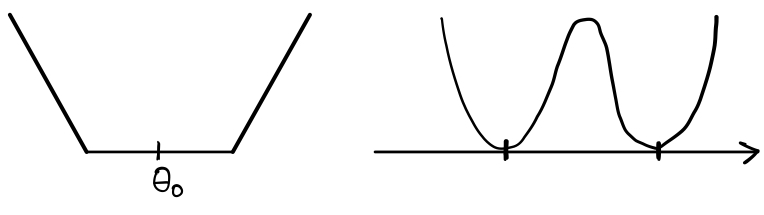
\includegraphics[scale=0.4]{wk1/1.jpg}  
    \end{figure} 

  \emph{Sufficient} conditions are given in \cref{lem:id}.

\subsubsection{Examples of Identification}
\begin{enumerate}
	\item \ul{\textbf{Maximum Likelihood}}:
	Let $f(W, \theta_0)$ be the true density. Then we have
	\begin{align*}
		Q(\theta_0) - Q(\theta) &= \E[-\log f(W, \theta_0) + \log f(W, \theta)] \\
								&= \E[\log (f(W, \theta)/f(W, \theta_0))] \\
								&\leq \log \E[f(W, \theta)/f(W, \theta_0)] \text{\tag{Jensen's Inequality}} \\
								&= \log \int \frac{f(W, \theta)}{\cancel{f(W, \theta_0)}}\cancel{f(W, \theta_0)}d\omega = \log (1) = 0 \text{\tag{Expectation is w.r.t true density}}
	\end{align*}
	Thus, $Q(\theta_0) - Q(\theta) \leq 0$ and this inequality is strict if $\Pr[f(W, \theta) \neq f(W, \theta_0)] > 0$ for all $\theta \neq \theta_0$. This is the same condition as required for \emph{point identification} of ML.
	\begin{itemize}
		\item \textbf{Misspecification:} When the true distribution of the data $f(W)$ is not in $\{f(W, \theta): \theta \in \Theta\}$, the ML estimator converges in probability to $\theta_0$ that uniquely minimizes the Kullback-Leibler (KL) divergence/information number, $K(f, f(\cdot, \theta))$, between the true density $f$ and the densities in $\{f(\cdot, \theta)\}_{\theta \in \Theta}$, where $K(f, f(\cdot, \theta)) = \E [\log f(W)] - \E [\log f(\cdot, \theta)]$.
	\end{itemize}
	%%%%%%%%%%%%% LEAST SQUARES %%%%%%%%%%%%%%%
	\item \ul{\textbf{Least Squares}}: Given $Y=g(X, \theta_0) + U$ and $\E[U|X] = 0$, 
	\begin{align*}
		Q(\theta) - Q(\theta_0) &= \E[(Y - g(X, \theta))^2 - (Y - g(X, \theta_0))^2]/2 \\
								&= \E[(g(X, \theta_0) + U - g(X, \theta))^2 - (U)^2]/2\\
								&= \E[(g(X, \theta_0) - g(X, \theta))^2 + 2U(g(X, \theta_0) - g(X, \theta)) + U^2 - U^2]/2\\
								&= \E[(g(X, \theta_0) - g(X, \theta))^2]/2 + 2\E[\E[U|X](g(X, \theta_0) - g(X, \theta))]/2\\
								&= \E[(g(X, \theta_0) - g(X, \theta))^2]/2 \geq 0
	\end{align*}
	The above inequality is strict if and only if $\Pr[g(X, \theta) \neq g(X, \theta_0)] > 0$ for all $\theta \neq \theta_0$.
	\begin{itemize}
		\item \textbf{Misspecification:} Suppose true conditional expectation is given by $\E[Y|X] = g(X)$ which is not in the family paramterized by $\theta \in \Theta$. Then,
		\begin{align*}
			Q(\theta) 	&= \E[(Y - g(X, \theta))^2]/2 \\
						&= \E[(Y - g(X) + g(X) - g(X, \theta))^2]/2 \\
						&= \E[(Y - g(X))^2]/2 + \E[(g(X) - g(X, \theta))^2]/2 + 2\E[(Y - g(X))(g(X) - g(X, \theta))]/2	\\
						&= \E[U^2]/2 + \E[(g(X) - g(X, \theta))^2]/2 + 2\underbrace{\E[U(g(X) - g(X, \theta))]}_{= 0\text{ as above}}/2	
		\end{align*}	
		Now, the estimated $\theta$ uniquely minimizes $\E[(g(X) - g(X, \theta))^2]$. This is the best mean-squared error approximation in the family $\{g(X, \theta): \theta \in \Theta\}$ to the conditional expectation function.
	\end{itemize}
	%------------------
	% GMM
	\item \ul{\textbf{GMM}}: By \hl{definition} of identification, $\theta_0$ is identified if $\E[g(W, \theta_0)] = 0$ \textbf{uniquely} at $\theta = \theta_0$ (The moment condition is not equal to zero at any other $\theta$). For identification, we also need the weighting matrix $A$ to be nonsingular.
	%------------------
	% Minimum Distance
	\item \ul{\textbf{Minimum Distance}}: If there exists a unique $\theta_0$ such that $\pi_0 = g(\theta_0)$ then identification assumption holds. Recall that $g(\cdot)$ is a known mapping from ``structural'' parameters $\theta$ to $\pi$, and minimum distance estimator minimizes the objective function $Q_n(\theta) = -[\hat{\pi}_n - g(\theta)]'A_n[\hat{\pi}_n - g(\theta)]/2$
	%------------------
	% Two-Step Estimators
	\item \ul{\textbf{Two-Step Estimators}}: \cref{ass:A3} satisfied if there exists a unique $\theta_0$ such that $G(\theta_0, \tau_0) = 0$.
	%------------------
	% Probit
	\item \ul{\textbf{Probit}}: Setup
	\begin{enumerate*}[(i)]
	\item $W = (Y, X)$,
	\item $Y \in \{0, 1\}$,
	\item $X \in \R^k$,
	\item $Y = \mathds{1}\{\epsilon \leq X'\theta\}$
	\item $\epsilon \perp X_i$
	\item $\epsilon \sim N(0,1)$
	\item $f^*(W) = f(W; \theta_0) = \Phi(X'\theta_0)^Y[1-\Phi(X'\theta_0)]^{1-Y}$
	\end{enumerate*} 

	To prove that identification holds, we need to show that $\forall \theta \neq \theta_0$, $\exists X$ s.t. $X'\theta \neq X'\theta_0$.
	\begin{claim}
	$\E[XX']$ exists and is nonsingular $\Rightarrow$ $\theta_0$ uniquely minimizes $Q(\theta)$.
	\end{claim}
	\begin{claimproof}
	Nonsingular $\E[XX']$ implies that it is positive definite. That is, for $\theta \neq \theta_0$,
	\begin{align*}
		\E[\{X'(\theta - \theta_0)\}^2] &= (\theta - \theta_0)'\E[XX'](\theta - \theta_0)>0\\
										&\Rightarrow X'(\theta - \theta_0) \neq 0 \\
										&\Rightarrow X'\theta \neq X'\theta_0
	\end{align*}
	where the last inequality simply means that $X'\theta$ and $X'\theta_0$ are \emph{not equal on a set of positive probability} -- that is, there exists some $X$ (with $\Pr = 1$) such that $X'\theta \neq X'\theta_0$ (if it was equal everywhere, the expectation will be zero). Both $\Phi(X'\theta)$ and $\Phi(-X'\theta)$ are strictly monotonic, so that $X'\theta \neq X'\theta_0$ implies both $\Phi(X'\theta) \neq \Phi(X'\theta_0)$ and $1-\Phi(X'\theta) \neq 1-\Phi(X'\theta_0)$, and hence $f(W; \theta) \neq f(W; \theta_0)$
	\end{claimproof}

\end{enumerate}


\subsubsection{Primitive Conditions for Identification}
\begin{lem}{}{id}
Let
\begin{enumerate}[noitemsep]
	\item $\Theta$ be compact.
	\item $Q(\theta)$ continuous, and
	\item $\theta_0$ uniquely minimizes $Q(\theta)$ over $\theta \in \Theta$
\end{enumerate}
Then, identification (\cref{ass:A3}) holds.
\end{lem}

\begin{figure}[htp]
\centering
\caption{All Three Conditions Must be Satisfied}
\label{fig:all3}
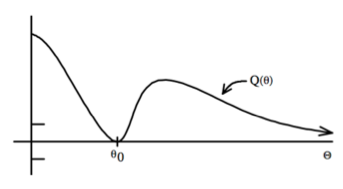
\includegraphics[width=.3\textwidth]{wk1/2}\hfill
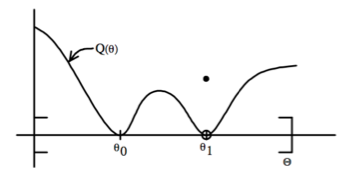
\includegraphics[width=.3\textwidth]{wk1/3}\hfill
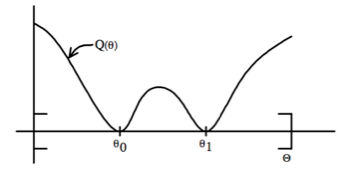
\includegraphics[width=.3\textwidth]{wk1/4}
\subcaption*{From left to right, violation of compactness, continuity, and uniqueness.}
\end{figure}
In the \hl{middle figure}, the $\inf$ condition is not satisfied at $\theta_1$.

\subsection{Main Result}
\begin{thm}{Consistency}{}\label{thm:consistency}
	\cref{ass:A1} (\textbf{EE}), \cref{ass:A2} (\textbf{UCONV}), and \cref{ass:A3} (\textbf{ID}) together imply consistency:
	$$\hat{\theta}_n \to^p \theta_0$$
\end{thm}

\begin{proof}
From \cref{ass:A3}, for a given $\epsilon > 0$, $\exists \delta > 0$ such that $$\theta \not \in B(\theta_0, \epsilon) \Rightarrow Q(\theta) - Q(\theta_0) \geq \delta > 0$$ 
Then,
\begin{align*}
\Pr[\hat{\theta}_n \not \in B(\theta_0, \epsilon)] 	&\leq \Pr[Q(\hat{\theta}_n) - Q(\theta_0) \geq \delta] \\
													&= \Pr[Q(\hat{\theta}_n) - Q_n(\hat{\theta}_n) + Q_n(\hat{\theta}_n) - Q(\theta_0) \geq \delta] \\
													&\leq \Pr[Q(\hat{\theta}_n) - Q_n(\hat{\theta}_n) + Q_n(\theta_0) + o_p(1) - Q(\theta_0) \geq \delta] \text{\tag{\cref{ass:A1}}} \\
													&\leq \Pr[2 \sup_{\theta \in \Theta} |Q_n(\theta) - Q(\theta)| \geq \delta] \to^p 0 \text{\tag{\cref{ass:A2}}}
\end{align*}
\end{proof}

\subsubsection{Extra: Primitive Conditions for Continuity of an Expectation}
$\E[m(W, \theta)]$ continuous if 
\begin{enumerate}[noitemsep]
\item $m(W, \theta)$ continuous in $\theta$ for all $W$
\item $\E[\sup_{\theta} \Vert m(W, \theta)\Vert] < \infty$
\end{enumerate}
$^*$Continuity is a weak assumption since kinks are allowed.


\section{Normality}


\end{document}